\documentclass[main.tex]{subfiles} % Subfile-Class


% ============================================================================== %
%                            Subfile document                                    %
% ============================================================================== %

\begin{document}

% Template

\subsubsection{Chassis und Fahrwerk}

Dieser Abschnitt behandelt die Evaluierung des Fahrwerks in Bezug auf die Radauswahl
und die Chassis-Konstruktion. Dabei werden verschiedene Konzeptlösungen diskutiert und
getestet. Abschliessend wird die finale Entscheidung auf Basis der Testergebnissen dokumentiert.

% ===================================================================================
\paragraph{Anforderungen}

\textbf{Gewicht:} \newline
Das Gewicht stellt, wie auch bei allen anderen Baugruppen, einen kritischen Faktor dar.
Daher soll das Chassis auf dem Konzept einer einzigen Grundplatte basieren, anstatt 
einen Volumenkörper zu entwerfen, der sämtliche Aktoren, Sensoren und Steuerungskomponenten
umschliesst. Zudem wird angestrebt, die Konstruktion auf zwei Räder zu beschränken.
Die Drehbewegung wird mittels Skid Steering realisiert. Um die Stabilität zu gewährleisten,
benötigt der Roboter jedoch einen dritten Auflagepunkt, dessen genaue Umsetzung in
verschiedenen Versuchen getestet werden muss.

\textbf{Geschwindigkeit:} \newline
Da die Motoren bereits ausgewählt sind und ihre Drehzahl technisch limitiert ist,
kann die maximale Fahrgeschwindigkeit lediglich über die Radgrösse definiert werden.
Von einem Getriebe wird bewusst abgesehen, um Gewicht und Kosten zu sparen.

\textbf{Kosten:} \newline
Das Chassis wird voraussichtlich mit einem 3D-Drucker gefertigt, da dem Team 25 Stunden
Druckzeit des HSLU-T\&A-Druckers kostenfrei zur Verfügung stehen. Die Kosten für die Räder
sollen unter 20 CHF bleiben, um ein grösseres Budget für kritische Funktionen bereitzustellen.

% ===================================================================================
\paragraph{Konzeptionierung}

Bereits früh in der Projektphase wurde entschieden, dass die Fortbewegung des Pfadfinders
mit zwei Rädern und einem dritten Auflagepunkt realisiert werden soll.
Abbildung~\ref{fig:Radkonzept} zeigt eine erste Konzeptskizze des Chassis, einschließlich
der Räder und einer Rutschfläche als dritten Auflagepunkt.

Durch die CAD-Konzeptionierung wurde ersichtlich, dass die Räder nicht breiter als 15 mm
sein dürfen, da sie sonst nicht auf der Welle des Schrittmotors montiert werden können.
Zudem müssen die Räder einen Mindestdurchmesser von 80 mm aufweisen, da andernfalls die
Liniensensoren nicht wie im Konzept vorgesehen montiert werden können. Alternativ könnten
die Sensoren höher positioniert werden, was jedoch eine Anpassung des Chassis und zusätzliche
Kosten erfordern würde, da die einfache Bodenplattenlösung nicht mehr umsetzbar wäre.

\begin{figure}[H]
    \centering
    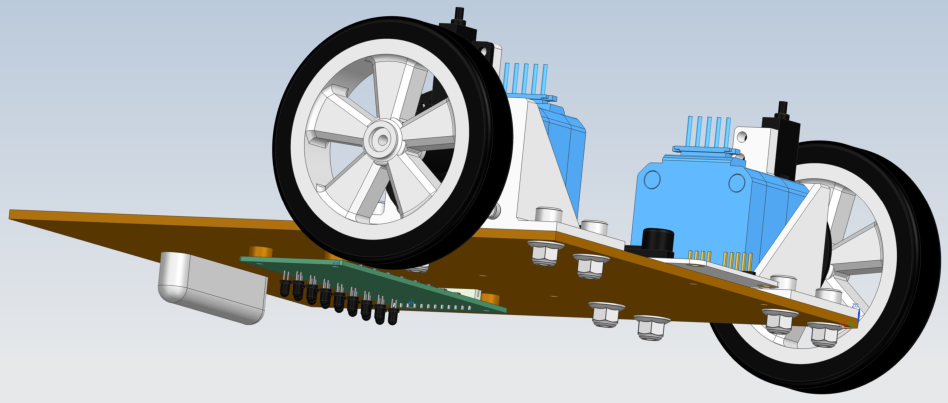
\includegraphics[width=0.75\textwidth]{Radkonzept.pdf}
    \caption{Chassis Konzept in Siemens NX}~\label{fig:Radkonzept}
\end{figure}

Auf Grundlage der genannten Anforderungen wurde auf verschiedenen Webseiten nach Rädern
gesucht, die eine passende Aufnahme für die Motorenwelle bieten. Unter Berücksichtigung
der Dimensionen wurde folgendes Rad ausgewählt:

\begin{table}[h]                                    % h = here
    \centering
    \begin{tabular}{|c|c|c|c|c|c|}                        % c=centered, l=left, r=right
        \hline
        Hersteller  & Herst. Nr.    & Preis     & Durchmesser   & Material      & Gewicht   \\
                    &               &           &               & Lauffläche    &           \\ \hline
        ServoCity   & 595660        & 9.05 CHF  & 80.3 mm       & Silikon       & 19 g      \\ \hline
    \end{tabular}
    \caption{Rad Parameter}
    \label{tab:Rad_Parameter}
\end{table}

Abbildung~\ref{fig:Rad_Vermassung} zeigt eine Detailzeichnung des gewählten Rades.
Ein grosser Vorteil dieses Rades gegenüber anderen Roboterrädern auf dem Markt ist
die Vielzahl an Montagepunkten an der Nabe. Dadurch kann mit relativ geringem Aufwand
ein Encoder angebracht werden, der die Erfassung von Schrittverlusten der
Schrittmotoren ermöglicht.

\begin{figure}[H]
    \centering
    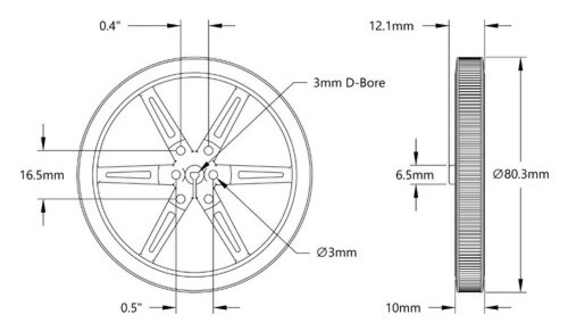
\includegraphics[width=0.75\textwidth]{Rad_Vermassung.pdf}
    \caption{Detailzeichnung ServoCity Rad}~\label{fig:Rad_Vermassung}
\end{figure}


% ===================================================================================
\paragraph{Versuche}
Versuche

% ===================================================================================
\paragraph{Entscheidung und Fazit}
Fazit und Entscheid

\end{document}
